One thing to have in mind when it comes to design, is colours, and it is very difficult to choose which colours to use when designing an interactive system. For example, Microsoft use blue in their Windows operating systems as an background colour, because blue means calm. And Apple also uses blue when it comes to their products. Considering Microsoft and Apple, it is most likely that every company has thought hard about what colours to use when it comes to designing their website. 
Another thing to have in mind is that the same colour can have a different meaning around the world. And example from \cite{DEBBook} is that the colour blue is seen as a bad thing for those working in healthcare and in business, because it means reliability.
In the table below one can see how the majority of the western world see what the different colours means. Figure \ref{Colors} shows this.

\begin{figure}[htb]
\centering
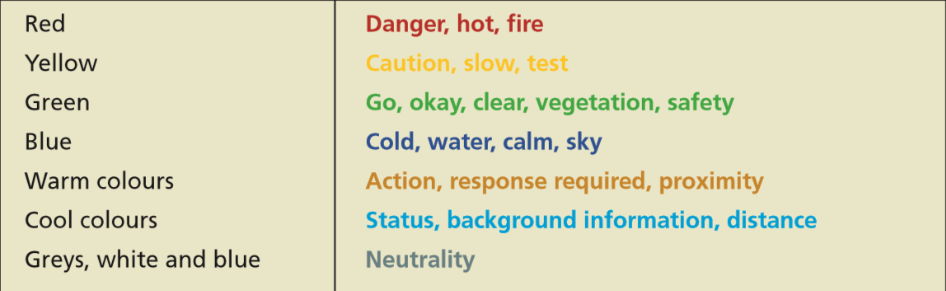
\includegraphics[width=0.8\textwidth]{Images/Colors.png}
\caption{Colors and the interactive meanings}
\label{Colors}
\end{figure}

In the Figure \ref{Login} considering this Login screen, which is the early version of it. We have tried to keep it simple and smooth and nothing to distract the user from doing what has to be done. It is simple because we only have few buttons and few interactions with the user. The colour we have chosen to our login screen is blue and white, which according to the table, are the right colours for the screen.

\begin{figure}[htb]
\centering
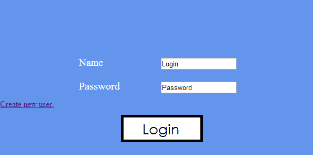
\includegraphics[width=0.6\textwidth]{Images/Login.png}
\caption{Design of the login screen}
\label{Login}
\end{figure}

When you have passed the login screen you come to our front page. Our front page is where you can go to everything that is relevant for the user. Again we have gone for a simple and clean look, there are only buttons which are necessary. It also has a profile image and the username besides it, to indicate that the user is logged in.

If we look at the sketch we made a long time ago in the start of the project it doesn't deviate too much from the product we have now. We have the same things with profile picture and username, but we have removed the option to insert a new media into ones medalist from the top bar. We have also removed the option to chat to others through the website, even though it was originally planned we wanted a chat system.
Instead of a home button that looks like a house in the lower right corner, we moved it up to take a more central placement and placed it on the top of the list of menu buttons. In that way it is more convenient for the user to come to the front place. The add media from the sketch, we have moved to the button medialist, which makes more sense and is more convenient. The central place where all the media is displayed, have stayed relatively the same, with a list that shows all the relevant media. Though, this have been collected into a single tab, for all recommendations given to the user. Again we have gone for the simple colours with blue and white. See Figure \ref{OldSite} for old design and Figure \ref{CurrSite} for the current design.

\begin{figure}[htb]
\centering
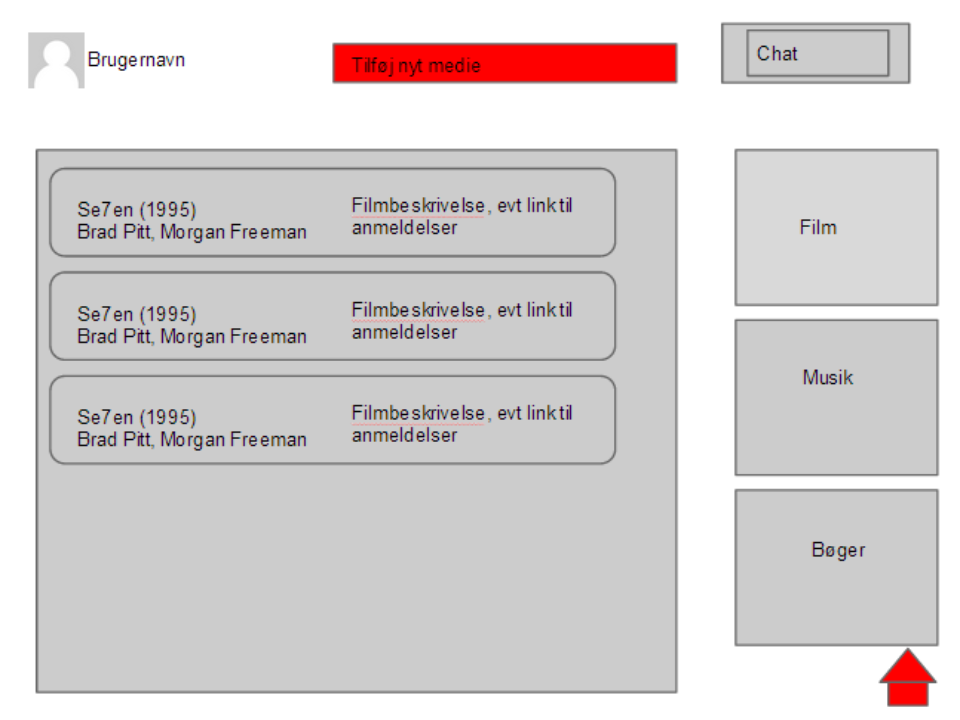
\includegraphics[width=0.8\textwidth]{Images/OldSite.png}
\caption{Early prorotype of the website design}
\label{OldSite}
\end{figure}


\begin{figure}[htb]
\centering
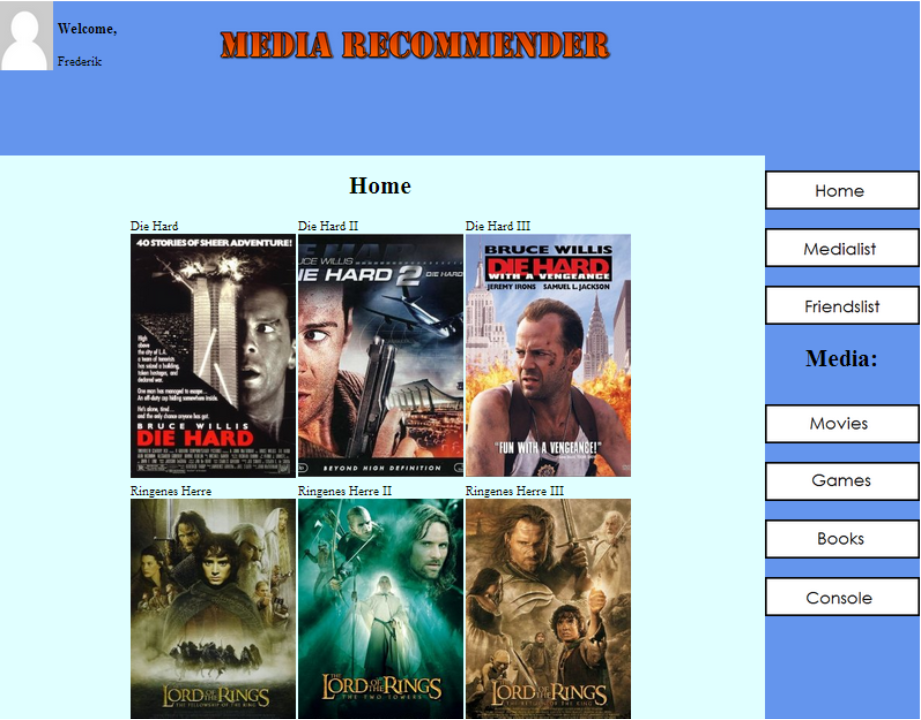
\includegraphics[width=0.8\textwidth]{Images/CurrSite.png}
\caption{Current version of the website design}
\label{CurrSite}
\end{figure}